\documentclass[12pt]{article}
\usepackage[spanish]{babel}
\usepackage[utf8]{inputenc}
\usepackage{amsmath}
\usepackage{listings}
\usepackage[usenames]{color}
\definecolor{gray97}{gray}{.97}
\definecolor{gray75}{gray}{.75}
\definecolor{gray45}{gray}{.45}
\definecolor{azul1}{RGB}{141,198,163}
\definecolor{azul2}{RGB}{24,107,122}
\definecolor{verde1}{RGB}{44,186,34}
\usepackage{graphicx}
\usepackage{caption}
\usepackage{subcaption}
\usepackage{textcomp}
\lstset{
        frame=Ltb,
        framerule=1pt,
        framextopmargin=3pt,
        framexbottommargin=3pt,
        framexleftmargin=0.6cm,
        framesep=0pt,
        rulesep=.4pt,
		backgroundcolor=\color{gray97},
		rulesepcolor=,
        tabsize=4,
        rulecolor=\color[RGB]{106, 182, 217}, %AZUL
        upquote=true,
        aboveskip={1.5\baselineskip}, %despues de la linea de texto
        columns=fixed,
        showstringspaces=false,
        extendedchars=true,
        breaklines=true,
        prebreak = \raisebox{0ex}[0ex][0ex]{\ensuremath{\hookleftarrow}},
        showtabs=false,
        showspaces=false,
        showstringspaces=false,
        basicstyle=\scriptsize\ttfamily\color[RGB]{39, 100, 46}, %Numeros de lineas, simbolos, puntos y coma y demas
        identifierstyle=\ttfamily\color[RGB]{56, 140, 189}, %variables
        commentstyle=\color[RGB]{62, 179, 101}, %comentarios
        stringstyle=\color[RGB]{247, 165, 42}, %impresiones
        keywordstyle=\bfseries\color[RGB]{237, 118, 150}, %funciones
        %
		numbers=left,
		numbersep=5pt,
		numberstyle=\tiny,
		numberfirstline = false,
		breaklines=true,
		}
\usepackage{graphicx}
\usepackage[colorinlistoftodos]{todonotes}
%\usepackage{natbib} %citas bibliograficas estilo APA :p
\usepackage{eso-pic}
\usepackage{avant}
\usepackage[top=2cm,bottom=2cm,left=2.5cm,right=3cm,headsep=8pt,a4paper]{geometry}
\usepackage{fancyhdr}
\pagestyle{fancy}
\fancyhf{}
%\fancyhead[LE,RO]{}
\fancyhead[RE,LO]{Teoría de Control II}
\fancyfoot[CE,CO]{\leftmark}
\fancyfoot[LE,RO]{\thepage}
\renewcommand{\headrulewidth}{2pt}
\renewcommand{\footrulewidth}{1pt}
\usepackage{hyperref}
\usepackage{tabu}
\usepackage{array}
\usepackage{multirow}
\usepackage{amssymb}
\usepackage{makeidx}
\graphicspath{ {images/} }
\usepackage{wrapfig}
\usepackage{enumerate}
\usepackage{amsmath,tikz}
\usetikzlibrary{matrix}
\usepackage{steinmetz}
\newcommand*{\horzbar}{\rule[0.05ex]{2.5ex}{0.5pt}}
\usepackage{calc}
\date{\today}

\begin{document}

\begin{titlepage}
\newcommand{\HRule}{\rule{\linewidth}{0.5mm}} 
\center
\textsc{\LARGE Universidad Nacional de San Antonio \\[0.2cm] Abad del Cusco}\\[1.5cm] 

\includegraphics[width=5cm]{escudo.jpg}\\[1cm]
\textsc{\Large Facultad de Ingeniería Eléctrica, Electrónica, Informática y Mecánica}\\[0.5cm] 
\textsc{\large Escuela Profesional de Ingeniería Electrónica}\\[0.5cm]
\HRule \\[0.4cm]
{ \huge \bfseries Modelamiento del Sistema\\\vspace{2mm}
Péndulo de Hélice}\\[0.4cm] 
\HRule \\[1.5cm]
\begin{minipage}{\textwidth}
\center 

\emph{Profesor:} \\
Roger Jesus Coaquira Castillo \\[1cm]

\begin{tabular}{ll}
\emph{Alumnos:} & \emph{Código:}\\
Heiner Brayan Companocca Huillca & 150418 \\
Luis Miguel Huachaca Hincho & 154870 \\
Hanan Ronaldo Quispe Condori & 163819 \\
Alfonso Alejandro Sevilla Hidalgo & 160345 \\
\end{tabular}
\end{minipage}\\[2cm]
\today
\end{titlepage}


\tableofcontents

\newpage
\section{Introducción}

El Péndulo de hélice es un péndulo el cual en la parte inferior de la varilla tiene una hélice, la cual ejerce una fuerza de empuje que hace mover el péndulo hacia arriba o abajo. Esta fuerza es utilizada para localizar el péndulo en un punto deseado respecto a la disponibilidad del ángulo mediante diferentes métodos de control. 
\\
Por la diversidad del sistema se puede aplicar diferentes métodos para el modelamiento, en este proyecto tomaremos en cuenta el modelamiento mediante Euler-Lagrange, lo que permite el aprendizaje y la profundización de esta técnica la cual considera las energías del movimiento sistemático, para la aplicación en sistemas independientes, completos y holonómicos \cite{MitLagrange}.
\\
El sistema es del tipo no-lineal por ende se desarrollará una linealización mediante un punto de equilibrio para la aplicación de los métodos accesibles de control. Un punto de equilibrio muy alejado al estado del controlador o si el sistema es extremadamente no-lineal hace que los diferentes métodos de control, no lleven a cabo el mantenimiento del sistema dinámico; por lo que el estudio de este comportamiento no lineal hace un importante significado para su análisis y sobre todo para su controlador. 

\\
Este tipo de sistema muestra un modelo de planta simple la cual es desarrollada y sirve como ejemplo para los modelos dinámicos dados en diferentes campos de la educación como en ingeniería electrónica, mecánica o mecátronica.
\newpage
\section{Modelamiento Matemático}
\\

\begin{figure}[h]
    \centering
    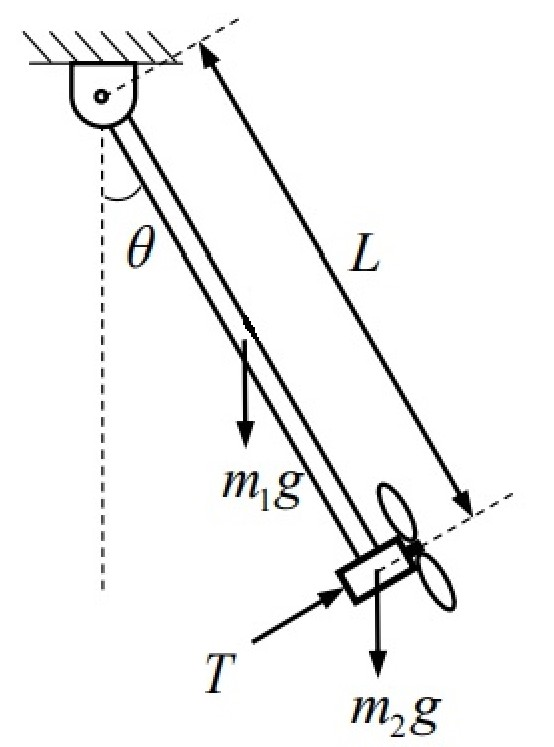
\includegraphics[width=8cm, height=9cm]{model.jpg}
    \caption{Sistema Péndulo Hélice}
    \label{fig:model}
\end{figure}

El sistema a modelar se muestra en la figura 1 \cite{taskin2017fuzzy}. Utilizando la metodología de Euler-Lagrange para el modelamiento,  se determinará primeramente el lagrangiano ($\mathcal{L}$) del sistema que está en función de la energía cinética ($\mathcal{K}$)   y potencial ($\mathcal{U}$) los cuales se calcularán a continuación.
\\
\\
\\
\textbf{Cálculo de Energía Cinética}

Se procederá a calcular las coordenadas cartesianas del extremo final  (cinemática directa cartesiana), por simple geometría se tendrá que la cinemática directa viene dada por:

%,en función de esta coordenada generalizada se tendrá la posición de reposo, este se encontrará en $\theta=0$, $\begin{bmatrix} x&y \end{bmatrix}^T=\begin{bmatrix} 0&-L \end{bmatrix}^T$, ádemas de esto se tendrá la posición del extremo en función de la coordenada generalizada $\theta$,  $\begin{bmatrix} x&y \end{bmatrix}^T=\begin{bmatrix} L\sen{\theta} & -L\cos{\theta} \end{bmatrix}^T$. 

\begin{equation}
    \begin{bmatrix}  x \\ y \\
    \end{bmatrix}=
    \begin{bmatrix} Lsen(\theta) \\ -L\cos(\theta)  \\
    \end{bmatrix}
    \label{eq:cin_direc}
\end{equation}

Para obtener la energía cinética del sistema se debe tener la velocidad de este, por lo cual se procederá a derivar la posición con respecto al tiempo.

\begin{equation}
    \frac{d}{dt}\begin{bmatrix}
        x \\
        y \\
    \end{bmatrix}=
    \begin{bmatrix}
        \dot{\theta}L\sen(\theta)  \\
        -\dot{\theta}L\cos(\theta)  \\
    \end{bmatrix}
    \label{eq:speed}
\end{equation}

El lagrangiano es una cantidad escalar, por lo que trabajaremos con el módulo de la ecuación (\ref{eq:speed}).

\begin{equation}
    \begin{split}
        \|v\|^2&=v.v^T=\sqrt{\dot{\theta}^2L^2sen^2{\theta}+\dot{\theta}^2L^2cos^2{\theta}}^2\\
        \|v\|^2&=L^2\dot{\theta}^2
    \end{split}
    \label{eq:speed_mod}
\end{equation}

La respectiva energía cinética asociada al sistema es:

\begin{equation}
    \begin{split}
        \mathcal{K} &= \frac{1}{2}mL^2\dot\theta^2\\
        \mathcal{K} &= \frac{1}{2}J\dot\theta^2\\
    \end{split}
    \label{eq:k}
\end{equation}

\textbf{Cálculo de la Energia Potencial}

La energía potencial considerando los centros de gravedad respectivos, la masa del péndulo ($m_1$) y la masa de la hélice ($m_2$), es:

\begin{equation}
    \begin{split}
        \mathcal{U} &=  -m_1g\frac{L}{2}\cos{\theta} -m_2gL\cos{\theta} \\
        \mathcal{U} &= -gL\cos{\theta(\frac{m_1}{2}+m_2)}
    \end{split}
    \label{u}
\end{equation}

\textbf{Cálculo del Lagrangiano}

El lagrangiano de un sistema, la cual proviene de la diferencia entre las energías, esta definido como:

\begin{equation}
    \mathcal{L}(q,\dot{q})=\mathcal{K}(q,\dot{q})-\mathcal{U}(q)
    \label{eq:lagran}
\end{equation}

Reemplazando las ecuaciones (\ref{eq:k}) y (\ref{u}) en el miembro derecho de \ref{eq:lagran} se tiene:

\begin{equation}
    \mathcal{L}(\dot{\theta},\theta)=\frac{1}{2}J\dot{\theta}^2+gL\cos{\theta}(m_2+\frac{m_1}{2})
\end{equation}

La ecuación de Euler-Langrange, se define como:

\begin{equation}
    \frac{d}{dt}(\frac{\partial \mathcal{L}(q,\dot{q})}{\partial\dot{q}})-\frac{\partial \mathcal{L}(q,\dot{q})}{\partial q}=\mathcal{Q}-f_f(\dot{q},f_e,\mathcal{Q})
    \label{eq:eu_lagran}
\end{equation}

Donde:

\begin{itemize}
    \item $q=[q_1,q_2,...,q_n]^T\in \mathrm{R}^n$: Es el vector de  coordenadas generalizadas.
    \item $\dot{q}=[\dot{q}_1,\dot{q}_2,...,\dot{q}_n]^T\in \mathrm{R}^n$: Es el vector de velocidades articulares.
    \item $\mathcal{Q}=[Q_1,Q_2,...,Q_n]\in \mathrm{R}^n$: Es el vector de fuerzas generalizadas aplicadas, donde el i-ésimo elemento $Q_i$ esta asociado con la i-ésima coordenada generalizada.
    \item $f_f(\dot{q},f_e,\mathcal{Q})\in \mathrm{R}^n$ es el vector de fuerzas de fricción.
\end{itemize}

Haciendo nuestra coordenada generalizada: $q={\theta}$ entonces,  $\dot{q}=\dot{\theta}$.
\\
Además, en la ecuación (\ref{eq:eu_lagran}) se puede deducir que la fuerza generalizada y la fuerza de fricción, respectivas son:

\begin{equation}
\begin{split}
    \mathcal{Q}&=\tau
    \\
    f_f(\dot{q},f_e,\mathcal{Q})&=c\dot{\theta}
\end{split}  
\label{eq:Q}
\end{equation}

Resolviendo las variables del miembro izquierdo de la ecuación de Euler-Lagrange (\ref{eq:eu_lagran}), se tiene:
\begin{equation}
    \begin{split}
        \frac{\partial \mathcal{L}}{\partial\dot{\theta}}&=J\dot{\theta}\\
        \frac{d}{dt}(\frac{\partial\mathcal{L}}{\partial\dot{\theta}})&=J\ddot{\theta}\\
        \frac{\partial \mathcal{L}}{\partial \theta }&=-Lg\sen(\theta)(m_2 + \frac{m_1}{2})\\
    \end{split}
    \label{eq:dq}
\end{equation}

Por lo que, reemplazando las ecuaciones (\ref{eq:Q}) y (\ref{eq:dq}) en la ecuación (\ref{eq:eu_lagran}) se obtiene el modelo dinámico Lagrangiano del sistema.  

\begin{equation}
    J\ddot{\theta}+Lg\sen(\theta)(m_2+\frac{m_1}{2})=\tau-c\dot{\theta}
    \label{eq:din_model}
\end{equation}

Para propositos de simulación de este modelo dinámico, se usaran los siguientes valores numéricos \cite{taskin2017fuzzy}.

\begin{table}[h!]
    \begin{center}
        \begin{tabular}{ |c|c|c| }
            \hline
            Parámetros & Unidades SI & Valor \\ 
            \hline
            $m_1$ masa del péndulo & kg & 0.21 \\
            $m_2$ masa del motor & kg & 0.16 \\
            $L$ longitud del péndulo & m & 0.6 \\
            $J$ momento de inercia del péndulo & $kgm^2$ & 0.083 \\
            $c$ coeficiente de amortiguamiento viscoso & $kgm^2/s$ & 0.074 \\
            $g$ gravedad & $m/s^2$ & 9.81 \\
            \hline
        \end{tabular}
        \caption{\label{tab:parametros}Parametros del modelo Matemático}
    \end{center}
\end{table}

Reemplanzando los valores numéricos la tabla \ref{tab:parametros} en la ecuación (\ref{eq:din_model}) y despejando la variable "$\ddot{\theta}&$ " se podrán hacer las siguientes simplificaciones.

\begin{equation}
    \begin{split}
        \ddot{\theta}&=\frac{\tau}{J}-\frac{c\dot{\theta}}{J}-\frac{Lg}{J}(m_2+\frac{m_1}{2})\sen(\theta)\\
    \ddot{\theta}&=12.04\tau-0.9\dot{\theta}-18.8\sen(\theta)
    \label{eq:eq_param}
    \end{split}
\end{equation}

Llevando a espacio de estados la ecuación (\ref{eq:eq_param}):

\begin{equation}
    \frac{d}{dt}
    \begin{bmatrix}
        \theta  \\
        \dot{\theta} \\ 
    \end{bmatrix}=\begin{bmatrix}
        \dot{\theta}  \\
        12.04\tau-0.9\dot{\theta}-18.8\sen(\theta) \\ 
    \end{bmatrix}
    \label{eq:state_space}
\end{equation}

En la ecuación (\ref{eq:state_space}) si hacemos que el valor del vector que contiene las variables de estado sea el valor "$0$", se podrá encontrar un valor de equilibrio como se muestra en a continuación.

\begin{equation}
    \begin{split}
        \begin{bmatrix}
            0  \\
            0  \\ 
        \end{bmatrix}&=\begin{bmatrix}
            \dot{\theta}  \\
            12.04\tau-0.9\dot{\theta}-18.8\sen(\theta) \\ 
        \end{bmatrix}\\
        \dot{\theta}&=0\\
        18.8sen(\theta)&=12.04\tau+0\\
        \theta&=arcsen(\frac{12.04\tau}{18.8})\\
        \text{tomando: } \tau&=1 \\
        \theta&=0.7rad\\
    \end{split}
    \label{eq:equilibrium}
\end{equation}

Este ultimo valor se usará como régimen de operación deseado al momento de linealizar el sistema ecuación  (\ref{eq:state_space}) ya que como se observa este no es lineal.
\\
\\
\textbf{Linealización del Sistema}

Se definirán los siguientes vectores para realizar esta linealización.

\begin{equation}
    \begin{split}
        F(\theta,\dot{\theta},\tau)&=\begin{bmatrix}
        \dot{\theta}  \\
        12.04\tau-0.9\dot{\theta}-18.8\sen(\theta) \\ 
        \end{bmatrix}\\
        \theta_o&=\begin{bmatrix} \theta _o & \dot{\theta}_o  \end{bmatrix}^T = \begin{bmatrix} 0&0  \end{bmatrix}^T \quad \text{Condiciones Iniciales}\\
        \theta_d&=\begin{bmatrix} \theta _d& \dot{\theta}_d  \end{bmatrix}^T \quad \text{Regimen de Operación Deseado}\\
        G(\theta,\dot{\theta},\tau)&=\theta
    \end{split}
    \label{eq:linearization}
\end{equation}

Linealizando el sistema se tendrá

\begin{equation}
    \begin{split}
        \frac{\partial F}{\partial \theta}&=\begin{bmatrix}
        0 & 1  \\
        -18.8\cos(\theta_d) & -0.9 \\ 
        \end{bmatrix}_{[\theta _d,\dot{\theta}_d]}\\
        \frac{\partial F}{\partial \tau}&=\begin{bmatrix}
        0 \\
        12.04 \\
        \end{bmatrix}\\
        y&=G\\
        y&=\theta\\
        y&=\begin{bmatrix}
        1 & 0 \\
        \end{bmatrix}
    \end{split}
    \label{eq:linearized}
\end{equation}

De la ecuación (\ref{eq:linearized}) podemos extraer el modelo del sistema en espacio de estados linealizado.

\begin{equation}
    \begin{split}
        \frac{d}{dt}
    \begin{bmatrix}
        \theta  \\
        \dot{\theta} \\ 
    \end{bmatrix}&=\begin{bmatrix}
        0 & 1  \\
        -18.8\cos{\theta_d} & -0.9 \\ 
    \end{bmatrix}
    \times
    \begin{bmatrix}
     \theta \\
      \dot{\theta} \\
      \end{bmatrix}+\begin{bmatrix}
     0 \\
     12.04 \\
      \end{bmatrix}\tau\\ 
      y&=\begin{bmatrix}
     1 & 0 \\
      \end{bmatrix}
      \begin{bmatrix}
     \theta \\
     \dot{\theta} \\
      \end{bmatrix}
    \end{split}
    \label{eq:lined_model}
\end{equation}

Reemplazando el punto calculado en la ecuación (\ref{eq:equilibrium}) se tendrá finalmente.

\begin{equation}
    \begin{split}
        \frac{d}{dt}
    \begin{bmatrix}
        \theta  \\
        \dot{\theta} \\ 
    \end{bmatrix}&=\begin{bmatrix}
        0 & 1  \\
        -14.379 & -0.9 \\ 
    \end{bmatrix}
    \times
    \begin{bmatrix}
     \theta \\
      \dot{\theta} \\
      \end{bmatrix}+\begin{bmatrix}
     0 \\
     12.04 \\
      \end{bmatrix}\tau\\ 
      y&=\begin{bmatrix}
     1 & 0 \\
      \end{bmatrix}
      \begin{bmatrix}
     \theta \\
     \dot{\theta} \\
      \end{bmatrix}
    \end{split}
    \label{eq:lined_model_no_constants}
\end{equation}
\newpage
\section{Simulación}

Para simular el sistema usaremos el método de Euler mediante derivadas con lo que podremos resolver la ecuación dinámica lineal; llevando la ecuación de espacio estado al modelo dinámico lineal del sistema.

\begin{equation}
    \begin{split}
    \ddot{\theta}+0.9\dot{\theta}+14.379\theta&=12.04\tau
    \label{eq:lin_ode}
    \end{split}
\end{equation}

Con la ecuación (\ref{eq:lin_ode}) se harán aproximaciones mediante derivadas obteniendo las siguientes reducciones de orden\cite{reyes:2020}.

\begin{equation}
    \begin{split}
        \theta(t)\backsimeq \thet(t_{k})\\
        \dot{\theta}(t)\backsimeq \dot{\theta}(t_{k})&=\frac{\theta(t_{k})-\theta(t_{k-1})}{h}\\
        \ddot{\theta}(t)\backsimeq\ddot{\theta}(t_{k})&=\frac{\dot{\theta}(t_{k})-\dot{\theta}(t_{k-1})}{h}=\frac{\frac{\theta(t_{k})-\theta(t_{k-1})}{h}-\frac{\theta(t_{k-1})-\theta(t_{k-2})}{h}}{h}\\
        \ddot{\theta}(t_{k})&=\frac{\theta(t_{k})-2\theta(t_{k-1})+\theta(t_{k-2})}{h^2}\\
    \end{split}
    \label{eq:euler_equivalent}
\end{equation}

La solución del modelo dinámico se obtendrá reemplazando las ecuaciones (\ref{eq:euler_equivalent}) en la ecuación (\ref{eq:lin_ode}).

\begin{equation}
    \begin{split}
        \theta(t_{k})&=\frac{12.04\tau+\lbrack\frac{2\times1}{h^2}+\frac{0.9}{h}\rbrack\theta(t_{k-1})-\frac{1}{h^2}\theta(t_{k-2})}{14.379+\frac{0.9}{h}+\frac{1}{h^2}}\\
    \end{split}
    \label{eq:eu_solution}
\end{equation}

Para implementar la solución discreta $\theta(t_{k})$ de la ecuación (\ref{eq:eu_solution}) se requieren los estados $\theta(t_{k-1})$,  $\theta(t_{k-2})$ y el periodo de muestreo $h$. Los estados pasados se pueden obtener considerando los estados previos del arreglo y el periodo de muestro según criterio.
\\
Esta simulación se ejecutará en un tiempo de $0$ a $10$ segundos con un periodo de muestreo de $10^{-3}$ segundos como se muestra en el código a continuación.

\lstinputlisting[language=Matlab]{eulers.m}

\section{Resultados}

%Se analizan los resultados de simulación obtenidos al ejecutar el %codigo mostrado.

\subsection{Escalon Unitario}

Luego de linealizar el sistema se obtuvo el modelo dinámico del sistema $12.04\tau=\ddot{\theta}+0.9\dot{\theta}+14.479\theta$, usando la transformada de Laplace se tendrá.

\begin{equation}
    \begin{split}
        s^2\theta(s)+0.9s\theta(s)+14.479\theta(s)&=12.04\tau(s)\\
        \theta(s)(s^2+0.9s+14.479)&=12.04\tau(s)\\
        \frac{\theta(s)}{\tau(s)}&=\frac{12.04}{s^2+0.9s+14.479}
    \end{split}
    \label{eq:transfer}
\end{equation}

En la ecuación (\ref{eq:transfer}) podemos ver observar una función de transferencia de segundo orden\cite[Página~165]{katsuhiko2010modern}.

\begin{equation}
    \begin{split}
        \frac{\theta(s)}{\tau(s)}&=\frac{12.04}{s^2+0.9s+14.479}=k\frac{\omega_n^2}{s^2+2\zeta\omega_n s+\omega_n^2}\\
    \end{split}
    \label{eq:compara}
\end{equation}

\begin{itemize}
    \item Ganancia $k=0.8$
    \item Frecuencia natural $\omega_n=3.7919$
    \item Factor de amortiguamiento $\zeta=0.118$
    \item Frecuencia de Oscilación $\omega_d=3.56rad$
\end{itemize}

Con estos parametros se podrá calcular la expresión analítica de la salida.

\begin{equation}
    \begin{split}
        \theta(t)&=\tau(t)k\lbrack1-e^{-\zeta\omega_n t}(cos(\omega_d t)+\frac{\zeta}{\sqrt{1-\zeta^2}}sen(\omega_d t))\rbrack\\
        \theta(t)&=\tau(t)0.8\lbrack1-e^{-0.45t}(cos(3.56t)+0.118sen(3.56t))\rbrack\\
        \textbf{Donde: }\tau(t)=1&\\
        \theta(t)&=0.8\lbrack1-e^{-0.45t}(cos(3.56t)+0.118sen(3.56t))\rbrack\\
    \end{split}
    \label{eq:salida}
\end{equation}

Podemos observar que el resultado analítico concuerda con el obtenido mediante la simulación el cual se muestra en la figura \ref{fig:escalon}.

\begin{figure}[h]
    \centering
    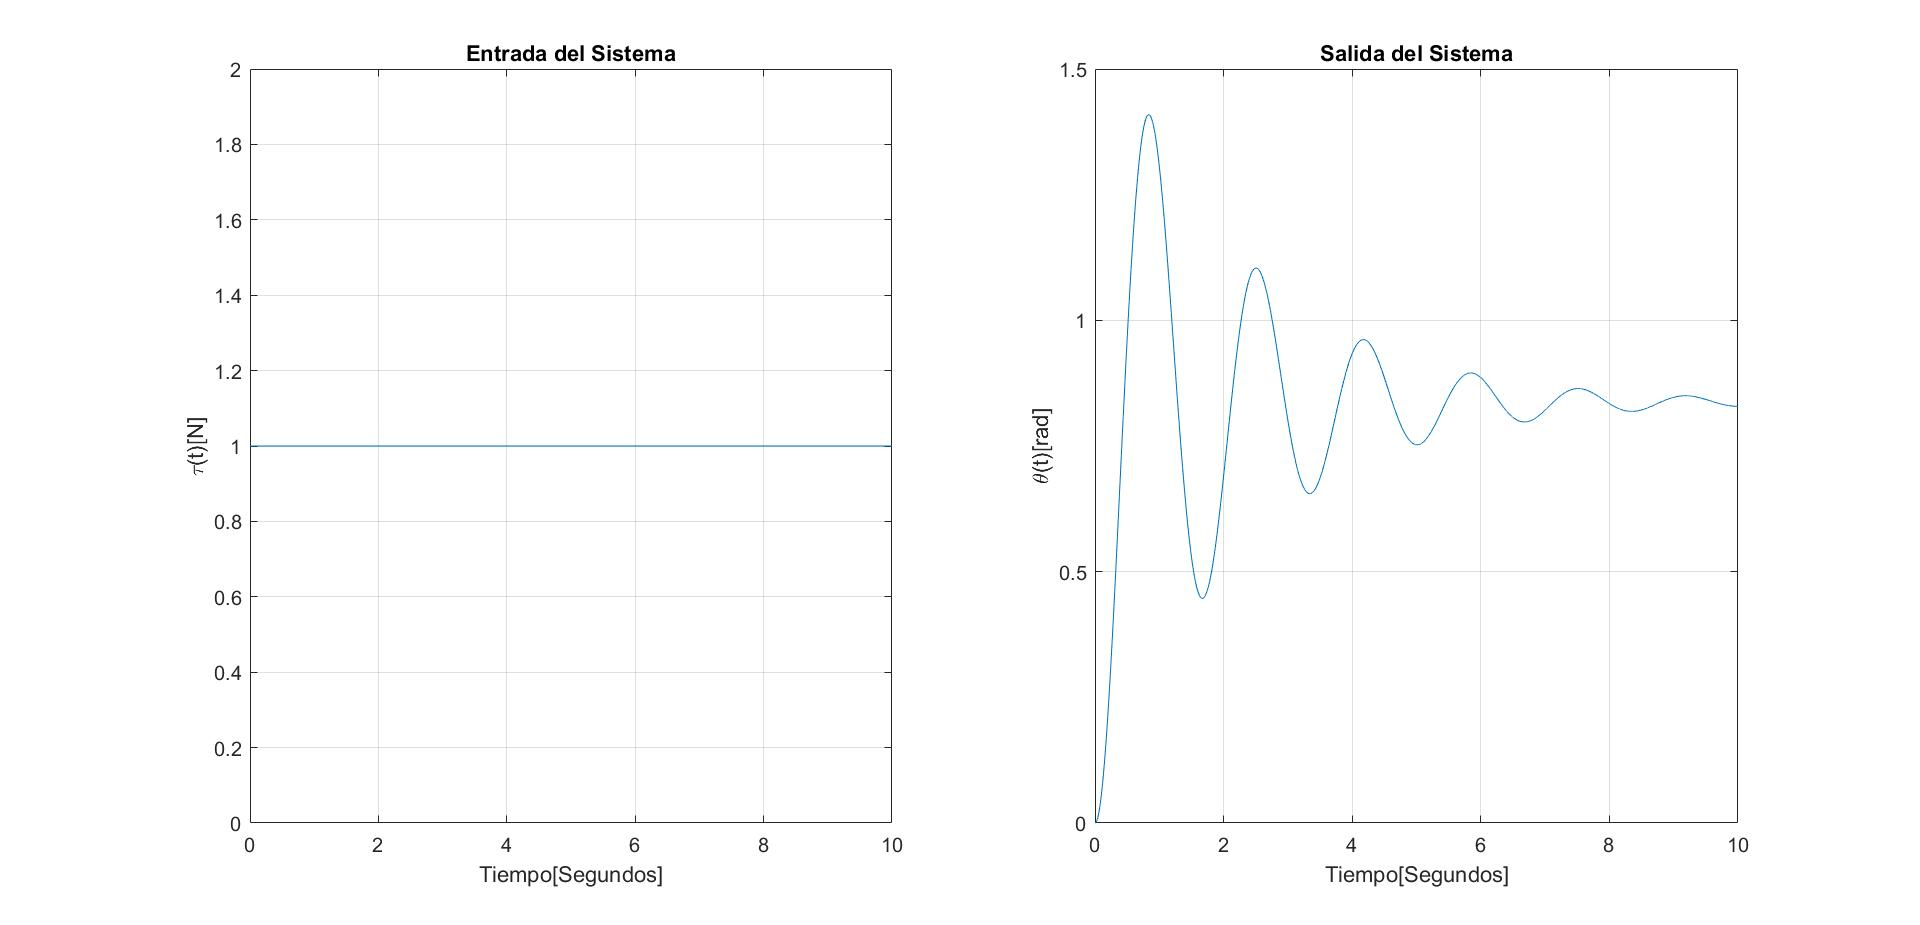
\includegraphics[width=17cm, height=5cm]{escalon.jpg}
    \caption{Entrada Escalon Unitario}
    \label{fig:escalon}
\end{figure}

\subsection{Senoidal}

En este caso se tendrá una entrada $\tau(t)=sen(2\pi t)$, con $f=1Hz$ y $T=1seg$ expresando como fasor la función de transferencia (\ref{eq:transfer}) se tendrá.

\begin{equation}
    \begin{split}
        \frac{\theta(s)}{\tau(s)}&=\frac{12.04}{s^2+0.9s+14.479}\\
        G(j\omega)&=\frac{12.04}{(j\omega)^2+0.9j\omega+14.479}\\
        G(j\omega)&=\frac{0.83}{\sqrt{(1-(\frac{\omega}{3.701})^2)^2+(0.06\omega)^2}}e^{-j tg^{-1}\begin{pmatrix} \frac{0.06\omega}{1-(\frac{\omega}{3.701})^2}\end{pmatrix}}\\
        \phi&=-tg^{-1}\begin{pmatrix} \frac{0.06\omega}{1-(\frac{\omega}{3.701})^2}\end{pmatrix}\\
        \text{Para }\omega=2\pi&\\
        \phi&=12.19046^\circ\approx 0.068\pi \quad |G(j\omega)|=0.51\\
    \end{split}
    \label{eq:fasor}
\end{equation}

La salida es

\begin{equation}
    \begin{split}
        \theta(t)&=\tau(t)|G(j\omega)|e^{j\phi}\\
        \theta(t)&=sen(2\pi t)|G(j\omega)|e^{j\phi}\\
        \theta(t)&=0.5sen(2\pi t+0.034seg)
    \end{split}
    \label{eq:sin_out}
\end{equation}

En la figura \ref{fig:sin} se puede observar una respuesta transitoria antes de que el resultado tome la forma de onda que se calculó analíticamente en la ecuación (\ref{eq:sin_out}).

\begin{figure}[h]
    \centering
    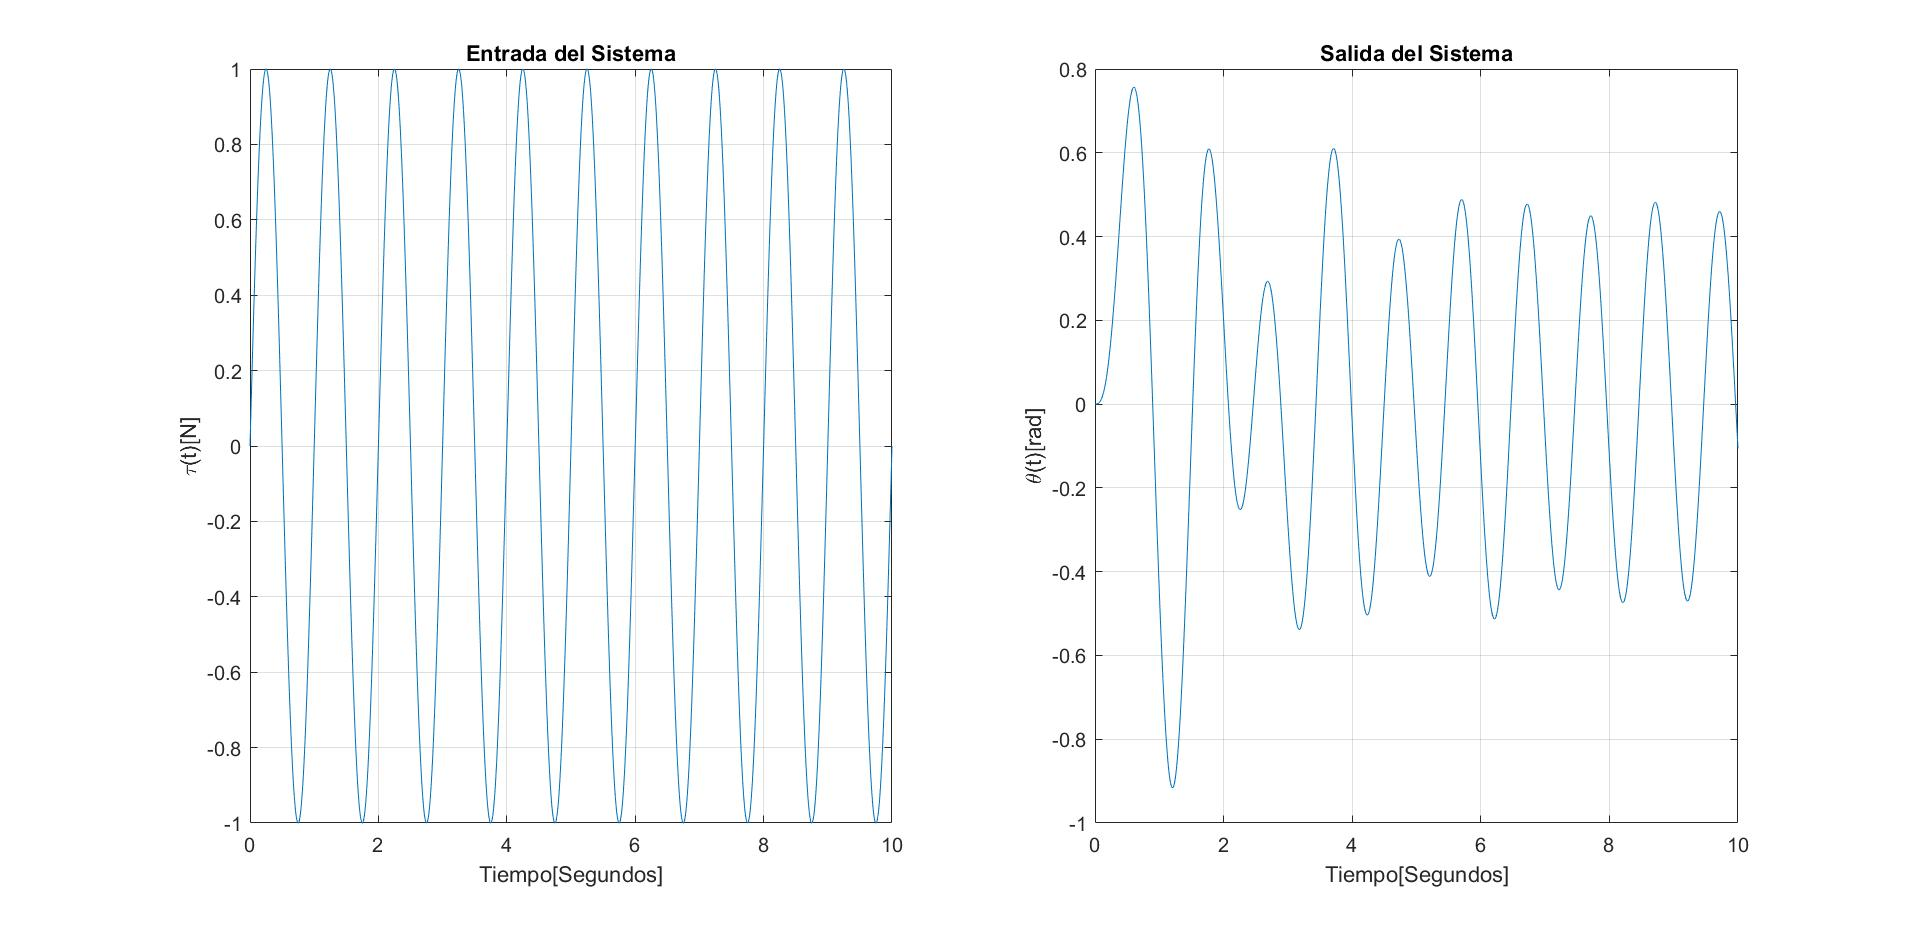
\includegraphics[width=17cm, height=7cm]{sin.jpg}
    \caption{Entrada Senoidal}
    \label{fig:sin}
\end{figure}

\newpage

\subsection{Impulso Retardado}
\vspace{6mm}
\begin{figure}[h]
    \centering
    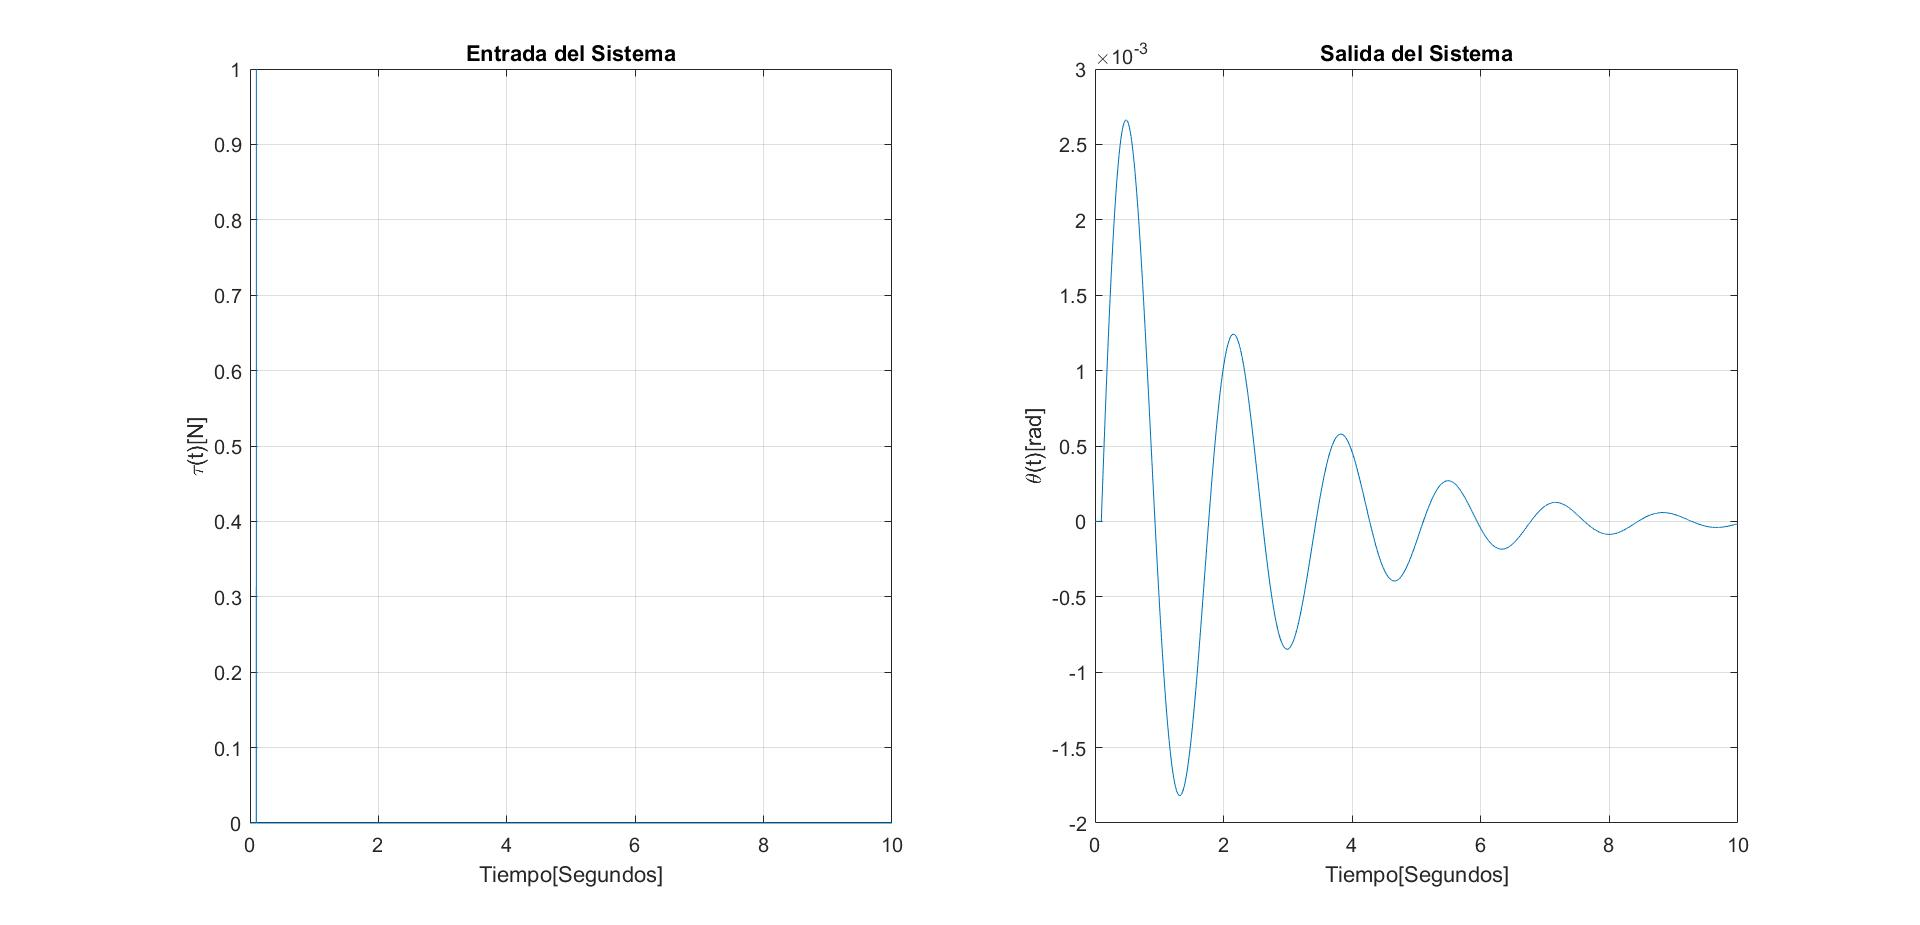
\includegraphics[width=17cm, height=7cm]{impulso.jpg}
    \caption{Entrada Impulso Unitario Retardado}
    \label{fig:step}
\end{figure}

En este caso la entrada es un impulso con el valor de $1$ en el instante $t=100mseg$, se puede observar que la salida tiene una pequeña salida en estado transitorio.

\subsection{Rampa Unitaria}

\begin{figure}[h]
    \centering
    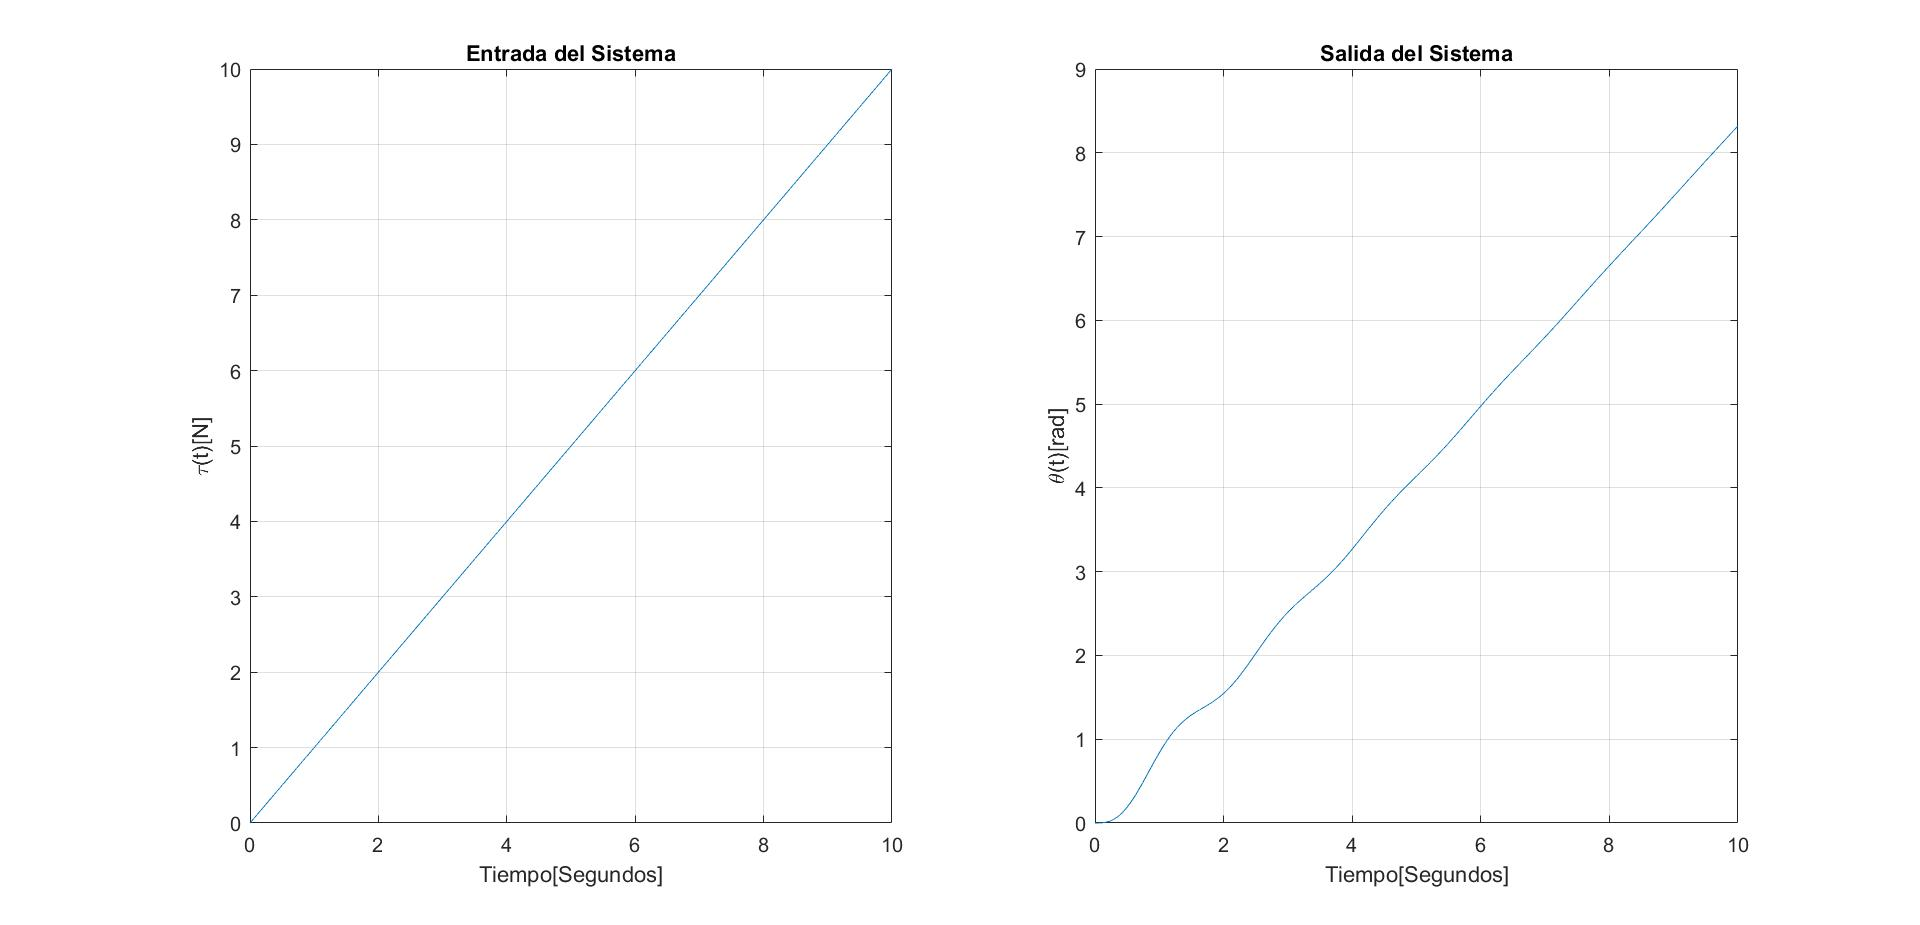
\includegraphics[width=17cm, height=7cm]{rampa.jpg}
    \caption{Entrada Rampa Unitaria}
    \label{fig:ramp}
\end{figure}

Por otro lado, considerando una entrada rampa podemos probar al sistema ante cambios que varien linealmente en el tiempo.
\newpage
\section{Conclusiones}
\begin{itemize}
    \item La ecuación Euler-Lagrange nos facilita la obtención de la ecuación diferencial (\ref{eq:eq_param}) del sistema, a partir de esto hallamos los ecuaciones de estado; de forma similar si se considera el sistema por las leyes de Newton se obtendra lo mismo.
    \item Con los parámetros del cuadro (\ref{tab:parametros}), se obtiene la ecuación (\ref{eq:eq_param}) que representa el cambio de estado en el tiempo, el cual muestra datos de entrada y salida.
    \item Con a la ecuación (\ref{eq:eq_param}) se puede deducir que la variable de salida es el ángulo, el cual nos permite colocarlo en cualquier punto arbitrariamente y la variable de entrada es el torque generado por la hélice, fuerza que mantiene en equilibrio el péndulo respecto al ángulo.
    \item Debido a las respuestas del escalon se puede apreciar que nuestro sistema presenta un tiempo de asentamiento prolongado y presenta un amortiguandoamiento con un sobre pico alto por lo que se optará por un controlador que haga el sistema menos amortiguado y que se estabilice en menor tiempo posible.
    \item La respuesta a una entrada de impulso oscila alrededor de cero y toma valores tanto positivos como negativos, entonces el sistema es subamortiguado.
    \item De la respuesta a la rampa se puede concluir que el error no es demasiado ya que la repuesta no se aleja tanto del paralelismo de la entrada.
\end{itemize}
\bibliographystyle{ieeetr}
\bibliography{references}
\end{document}